Quelle: \href{http://drops.dagstuhl.de/opus/volltexte/2015/4944/pdf/44.pdf}{Visibly Counter Languages
and Constant Depth Circuits}

Was wir von reg. Sprachen wissen:
\begin{itemize}
\item $REG$ ist $NC^1$-vollst.
\item $REG\cap AC^0 = FO[Reg.]$
	= quasi aper. $\gamma:\Sigma^*\to Synt(L)$
\item $REG L \notin AC^0 \Rightarrow L \text{ ist } ACC^0 \text{-schwer}$
\end{itemize}
$AC^0 \subsetneq ACC_k^0 \subseteq TC^0 \subseteq NC^1 \subseteq L \subseteq NL$\\
\vspace{1cm}\\
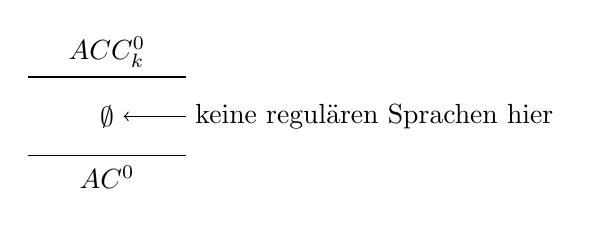
\begin{tikzpicture}
\draw (0,1) -- (2,1) node[midway, above] (acc) {$ACC_k^0$};
\node at (1,0.5) (empty) {$\emptyset$};
\draw [<-] (empty) -- (2,0.5) node [anchor= west] {keine regulären Sprachen hier};
\draw (0,0) -- (2,0) node[midway, below] (ac0) {$AC^0$};
\end{tikzpicture}\\
Dichotomie\\
VPL auch $NC^1$-vollständig, also auch $VCL$.

\section{Definition}
$k-VCA\quad\mathcal{A} = (Q, q_0, E, \Sigma, \delta_0, \dots, \delta_k)$\\
$$\delta_i = Q \times \Sigma \to \Sigma$$
Akz: Endzust. in Lauf erreichbar: $\delta_{min}(m, \Delta(w))$ wird angewandt, nachdem $w$ gelesen wurde.\\
\begin{tikzpicture}
\draw[->] (0,0) -- (0,3);
\node at (0,1) [anchor=east] (m) {$\delta_m$};
\draw[dotted] (m) -- (4,1);
\draw[gray!50] (0,0) -- (1,2) -- (2,1) -- (3,3) -- (4,0);
\fill[gray!20, pattern=north east lines] (0.5,1) -- (1,2) -- (2,1) -- (3,3) -- (3.667,1) -- cycle;
\draw[->] (0,0) -- (4,0);
\end{tikzpicture}\\
$$\Delta(w) = |w|_{call} - |w|_{return}$$
{\bf Bsp.:}\\ $a^nb^n \to 1-VCL$\\
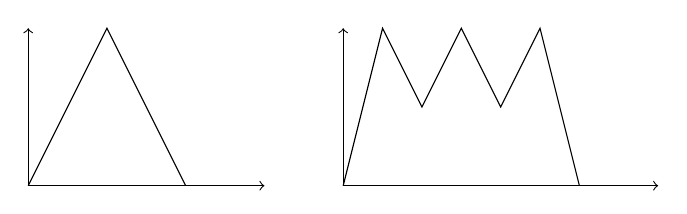
\begin{tikzpicture}
	\draw[->] (0,0) -- (0,2);
	\draw[->] (0,0) -- (3,0);
	\draw (0,0) -- (1,2) -- (2,0);

	\draw[->] (4,0) -- (4,2);
	\draw[->] (4,0) -- (8,0);
	\draw (4,0) -- (4.5,2) -- (5,1) -- (5.5,2) -- (6,1) -- (6.5,2) -- (7,0);
\end{tikzpicture}\\
\vspace{0.5cm}
$a^nb^{n-3}a^mb^{m+3} \to 4-VCA$\\
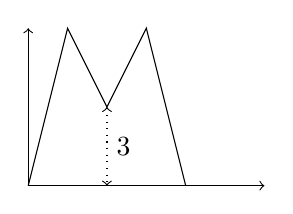
\begin{tikzpicture}
	\draw[->] (0,0) -- (0,2);
	\draw[->] (0,0) -- (3,0);
	\draw (0,0) -- (0.5,2) -- (1,1) -- (1.5,2) -- (2,0);
	\draw[<->,dotted] (1,1) -- (1,0) node[midway, right] {$3$};
\end{tikzpicture}\\
\vspace{1cm}\\
Nicht in $AC^0$: $\mathbb{D}$, da $TC^0$-schwer,\\
$MAJ,EQU$\\
{\bf Bsp.:} $L = (a|aba)^nb^n$ $TC^0$-schwer\\
{\bf Beweis:} zeige $EQU \leq AC^0 L$\\
\begin{flalign*}
	f&\in AC^0 \text{ mit } w \in EQU \Leftrightarrow f(w)\in L&\\
	f(w)&= \varphi(w)\Psi(w)\quad \varphi, \Psi \text{ Homs.}&\\
	\varphi(a) &= aaa&\\
	\varphi(b) &= aba\quad \Psi(w)= b^{2|w|}&\\
\end{flalign*}
Zu viele $a$'s: 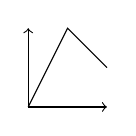
\begin{tikzpicture}\draw[->] (0,0) -- (1,0); \draw[->] (0,0) -- (0,1);\draw (0,0) -- (0.5,1) -- (1,0.5);\end{tikzpicture}$\quad$
zu viele $b$'s: 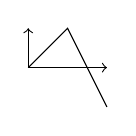
\begin{tikzpicture}\draw[->] (0,0.5) -- (1,0.5); \draw[->] (0,0.5) -- (0,1);\draw (0,0.5) -- (0.5,1) -- (1,0);\end{tikzpicture}
\begin{flalign*}
	|w|_a &= |w|_b \rightarrow |f(w)|_a = \frac{3|w|}{2} + \frac{2|w|}{2} > \frac{5}{2}|w|&\\
	|f(w)|_b &= \frac{|w|}{2} + 2|w| = \frac{5}{2}|w|&\\
\end{flalign*}
\section{Was macht L schwer?}
$\rightarrow$ Variable Steigung\\
Bsp. kann verallgemeinert werden
\subsection{Definition}
Zustand q hat \underline{konstante Steigung}, wenn $\exists \alpha \in \mathbb{Q}$ ($\alpha$: Steigung) $\forall w \in \Sigma^*$ mit $$ (q,h_1) \xrightarrow{w} (q,h_2)\text{ und}$$
$\forall w'$ Präfix von $w: h_1 + \Delta(w') \geq m$ gilt:
$$h_2 = \alpha|w|+h_1 \text{ Steigung}$$
\begin{tikzpicture}
	\tikzstyle{dot}=[draw,circle,fill = black, inner sep=0pt,minimum size=2pt]
	\draw[->] (0,0) -- (5,0);
	\draw[->] (0,0) -- (0,5);
	\draw (0,1) -- (-0.1,1) node [left] {$m$};
	\draw (0,2) -- (-0.1,2) node [left] {$h_1$};
	\draw (0,4) -- (-0.1,4) node [left] {$h_2$};
	\node[dot,right] at (1,2) {};
	\node[dot,right] at (4,4) {};
	\draw[dashed] (1,2) -- (4,4) node [midway,below] {$\alpha$};
	\draw plot[smooth] coordinates {(1,2) (1.8,1.6) (2, 3) (2.5, 4) (3,3.5) (3.7, 3.5) (4,4)};
	\node[left] at (1,2) {$q$};
	\node[right] at (4,4) {$q$};
\end{tikzpicture}
